
\documentclass[11pt]{article}
\usepackage[paper=letterpaper]{geometry}
\pdfpagewidth 8.5in
\pdfpageheight 11in
\setlength\parindent{0in}

%% AMS PACKAGES - Chances are you will want some or all of these if writing a math dissertation.
\usepackage{amsmath, amscd, amssymb, amsthm, multirow, enumerate, multicol, graphicx}
\DeclareGraphicsExtensions{.jpg}
\newcommand{\Z}{\mathbb{Z}}
\newcommand{\R}{\mathbb{R}}
\newcommand{\Q}{\mathbb{Q}}
\newcommand{\C}{\mathbb{C}}
\newcommand{\N}{\mathbb{N}}
\newcommand{\V}{\mathbb{V}}
\newcommand{\U}{\mathcal{U}}
\newcommand{\del}{\partial}
\newcommand{\real}{\textrm{Re }}
\newcommand{\imag}{\textrm{Im }}
\newcommand{\pd}[2]{\frac{\partial #1}{\partial #2}}
\newcommand{\deriv}[2]{\frac{d #1}{d #2}}
\newcommand{\sumk}{\sum_{k=1}^\infty}
\newcommand{\sumj}{\sum_{j=1}^\infty}
\newcommand{\sumn}{\sum_{n=0}^\infty}
\newcommand{\summ}[2]{\sum_{k=#1}^{#2}}
\newcommand{\sig}[1]{\sum_{#1 =1}^\infty}
\newcommand{\un}[1]{\bigcup_{#1 =1}^\infty}
\newcommand{\inter}[1]{\bigcap_{#1 =1}^\infty}
\newcommand{\ip}[2]{\langle #1, #2 \rangle}
\newcommand{\ipxu}{\langle x,u_j \rangle}
\newcommand{\uj}{\{u_j\}_{j=1}^\infty}
\newcommand{\B}{\mathcal{B}}

\newcommand{\Example}{\noindent {\bf Example. \quad} }
\newcommand{\Proof}{\noindent {\bf Proof: \quad} }
\newcommand{\Remark}{\noindent {\bf Remark. \quad} }
\newcommand{\Remarks}{\noindent {\bf Remarks. \quad} }
\newcommand{\Case}{\noindent {\underline{Case} \quad} }

\newcommand{\st}{ \; \big | \:}

\newcommand{\deuc}{d_{\mathrm euc}}
\newcommand{\dtaxi}{d_{\mathrm taxi}}
\newcommand{\ddisc}{d_{\mathrm disc}}
\newtheorem{theorem}{Theorem}[section]
\newtheorem{lemma}[theorem]{Lemma}
\newtheorem{proposition}[theorem]{Proposition}
\newtheorem{corollary}[theorem]{Corollary}
\theoremstyle{definition}
\newtheorem{definition}[theorem]{Definition}
\newtheorem{example}[theorem]{Example}

\begin{document}
Homework 1 \hfill Aaron Maurer
\hrule
\begin{enumerate}
    \item[1.]
        \begin{enumerate}
            \item[a)]
                \textbf{Task:} Prove that $RSS = SYY - \frac{(SXY)^2}{SXX}$
                \begin{align*}
                    RSS &= \sum_{i=1}^n \left [y_i - (\hat{\beta}_0 + \hat{\beta}_1 x_i) \right ]^2
                    \\ &= \sum_{i=1}^n \left [y_i - (\bar{y} - \hat{\beta}_1 \bar{x} + \hat{\beta}_1 x_i) \right ]^2 
                    \\ &= \sum_{i=1}^n \left [y_i - \bar{y} + \frac{SXY}{SXX} \bar{x} - \frac{SXY}{SXX} x_i \right ]^2
                    \\ &= \sum_{i=1}^n \left [(y_i - \bar{y}) - \frac{SXY}{SXX} (x_i - \bar{x}) \right ]^2
                    \\ &= \sum_{i=1}^n \left [(y_i - \bar{y})^2 - 2 \frac{SXY}{SXX}(y_i - \bar{y})(x_i - \bar{x}) + \left(\frac{SXY}{SXX}\right)^2 (x_i - \bar{x})^2 \right ]
                    \\ &= \sum_{i=1}^n (y_i - \bar{y})^2 - 2 \frac{SXY}{SXX}\sum_{i=1}^n (y_i - \bar{y})(x_i - \bar{x}) + \left(\frac{SXY}{SXX}\right)^2 \sum_{i=1}^n (x_i - \bar{x})^2
                    \\ &= SYY - 2\frac{SXY}{SXX}SXY + \left(\frac{SXY}{SXX}\right)^2SXX
                    \\ &= SYY - \frac{SXY^2}{SXX}
                \end{align*}
            \item[b)]
                \textbf{Task:} Use Cauchy-Schwarz to prove that RSS is nonnegative.
                \begin{align*}
                    RSS &= SYY - \frac{SXY^2}{SXX}
                    \\ &=  \|y-\bar{y}\|^2 - \frac{\langle x - \bar{x}, y - \bar{y} \rangle^2}{\|x-\bar{x}\|^2}
                    \\ &\geq \|y-\bar{y}\|^2 - \frac{\|x-\bar{x}\|^2 \|y-\bar{y}\|^2}{\|x-\bar{x}\|^2}
                    \\ &\geq \|y-\bar{y}\|^2 - \|y-\bar{y}\|^2
                    \\ &\geq 0
                \end{align*}
        \end{enumerate}
    \item[2.]
        \textbf{Task:} Show that linear regression and k-nearest neighbor regression are both of the class $\hat{f}(x_0)=\sum_{i=1}^N l_i(x_0;\mathcal{X})y_i$. \\
        Linear regression is a model of the form: \\
        \begin{align*}
            \hat{f}(x_0) &= \hat{\beta}_0 + \hat{\beta}_1 x_0
            \\ &= \bar{y} - \hat{\beta}_1 \bar{x} + \hat{\beta}_1 x_0
            \\ &= \bar{y} + (x_0 - \bar{x})\frac{SXY}{SXX}
            \\ &= \bar{y} + (x_0 - \bar{x})\frac{\sum_{i=1}^N (x_i - \bar{x})y_i}{SXX}
            \\ &= \bar{y} + \sum_{i=1}^N \frac{(x_0 - \bar{x})(x_i - \bar{x})}{SXX}y_i
            \\ &= \sum_{i=1}^N \left [ \frac{(x_0 - \bar{x})(x_i - \bar{x})}{SXX}y_i + \frac{\bar{y}}{N} \right ]
            \\ &= \sum_{i=1}^N \left [ \frac{(x_0 - \bar{x})(x_i - \bar{x})}{SXX} + \frac{1}{N} \right ]y_i
        \end{align*}
        Accordingly, it is of the desired form for 
        \[ l_i(x_0;\mathcal{X})=\frac{(x_0 - \bar{x})(x_i - \bar{x})}{SXX} + \frac{1}{N} \]
        Nearest neighbors regression is trivially of that form, with $N_{k,i}$ being the set of $k$ $x_j$ closest to $x_0$:
        \[ l_i(x_0;\mathcal{X})=\frac{I_{N_{k,x_0}}(x_i)}{k} \]
    \item[3.]
        Please note that all work is in the R supplement
        \begin{enumerate}
            \item[2.1.1]
                \\ 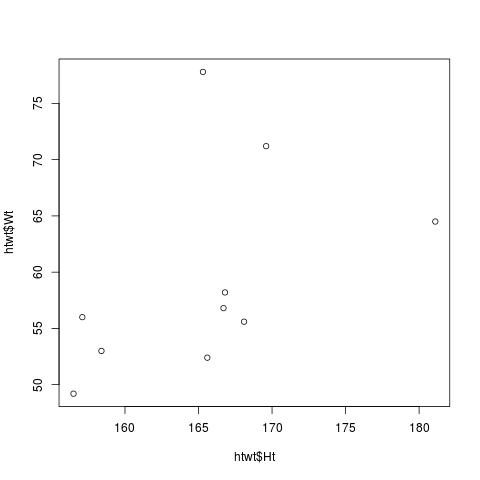
\includegraphics[width=8cm]{hw1_2_1_1} \\ 
                I would argue that this data, though seeming to indicate some sort of correlation bet ween height and weight befitting a linear model, is too small considering the amount of noise for a linear regression to make sense. The estimates would be far too noisy to read anything into it. That said, if there was more data it looks like a linear model would probably make sense.
            \item[2.1.2]
                See the R output for the calculation and confirmation of most of the values. 
                \[ \hat{\beta}_1=.582, \hat{\beta}_0=-36.876, \]
                \\ 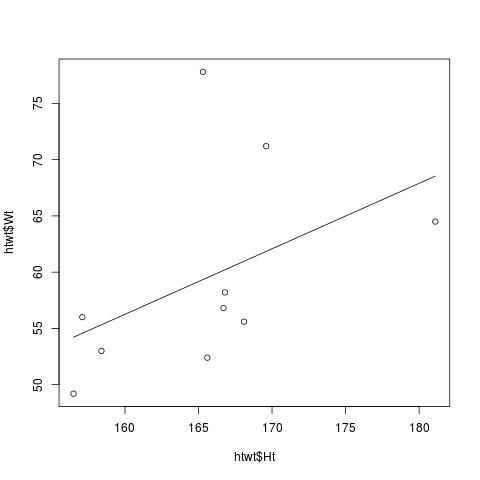
\includegraphics[width=8cm]{hw1_2_1_2} \\ 
            \item[2.1.3]
            \[\sigma^2=71.502, se(\hat{\beta}_1)=.389, se(\hat{\beta}_0)=64.473, Cov(\beta_0,\beta_1)=-25.070 \] 
            \[t_{\beta_1} = 1.496, t_{\beta_0}=-94.752, p_{\beta_1} = .173, p_{\beta_0} = 1.718e-13 \]
            \item[2.1.4]
                \begin{center}
                    \begin{tabular}{r | r r r r r}
                        Regression & df      & ss      & ms      & F     & pval \\
                        \hline
                        Regression & 1       & 159.947 & 159.947 & 2.237 & \approx 0 \\
                        Residual   & 8       & 572.014 & 71.502  &       &  \\
                        Total      & 731.961 &         &         &       & 
                    \end{tabular}
                \end{center}
                t_{\beta_1}^2 = 2.239 = F
        \end{enumerate}
        
    \item[4.]
        Please note hat all work is in the R supplement
        \begin{enumerate}
            \item[b)]
                While certain variables seem to be approximately normally distributed, such as pH, others seem to be very distinctly not normally distributed, such as alcohol. 
                \\ \includegraphics[width=8cm]{hw1_4b_pH} \\ 
                \\ 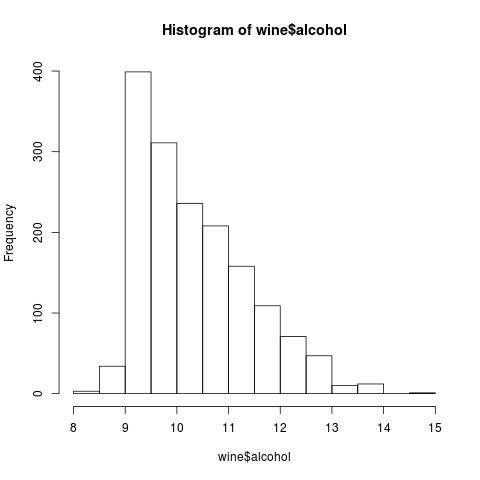
\includegraphics[width=8cm]{hw1_4b_alcohol} \\
                We also see some variables that clearly have a strong correlation, such as density and fixed.acidity, while with others like alcohol and citric.acid, if there is a correlation is hardly obvious.
                \\ 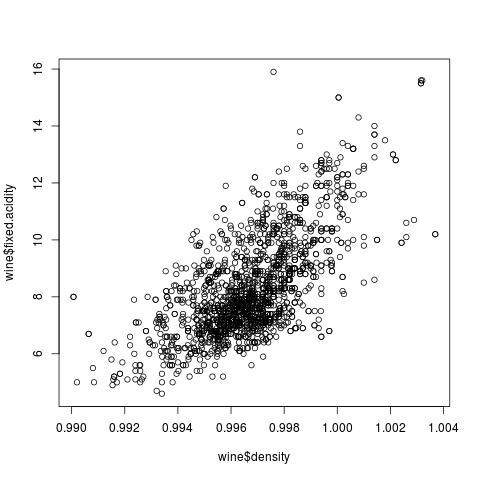
\includegraphics[width=8cm]{hw1_4den_to_acid} \\ 
                \\ 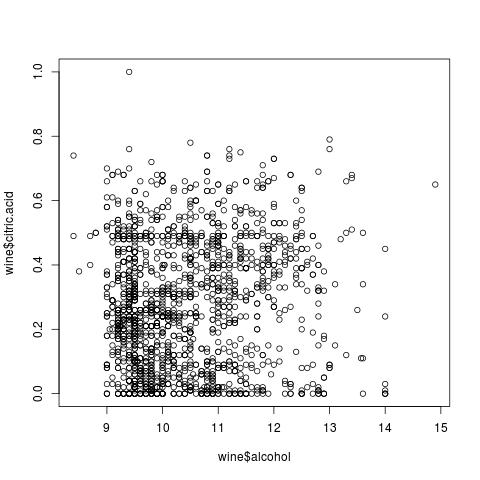
\includegraphics[width=8cm]{hw1_4alc_to_cit} \\
                Also, quality is clearly a categorical, rather than truly continuous.
            \item[c)]
                \\ \includegraphics[width=8cm]{hw1_4c} \\
                Most of these pairwise relationships at least seem to indicate some kind of correlation based on eyeballing the plot. pH and density look the closest to being independent, though there may be a very weak negative correlation. citric.acid and density look like they at best have a weak positive correlation. Its hard to tell if the correlations are linear, but they look to be at worst a little bit curved, such as in the case of fixed.acidity and pH, which can be modeled with a linear model
                \\ 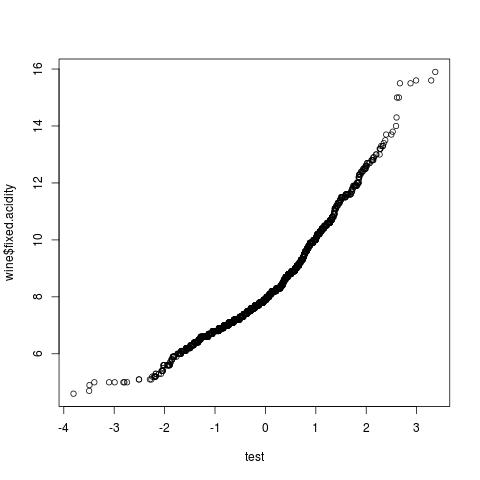
\includegraphics[width=8cm]{hw1_4c_fixed_acidity} \\
                \\ \includegraphics[width=8cm]{hw1_4c_pH} \\
                \\ 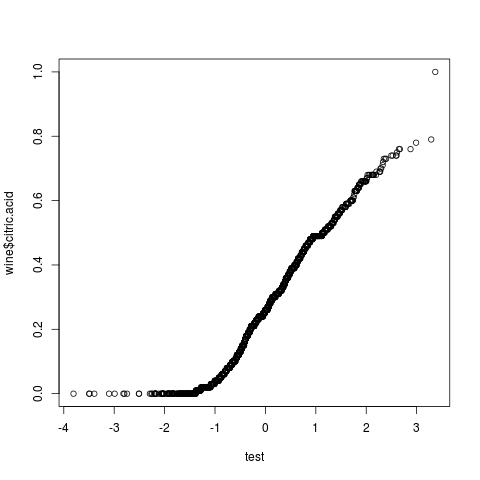
\includegraphics[width=8cm]{hw1_4c_citric_acid} \\
                \\ 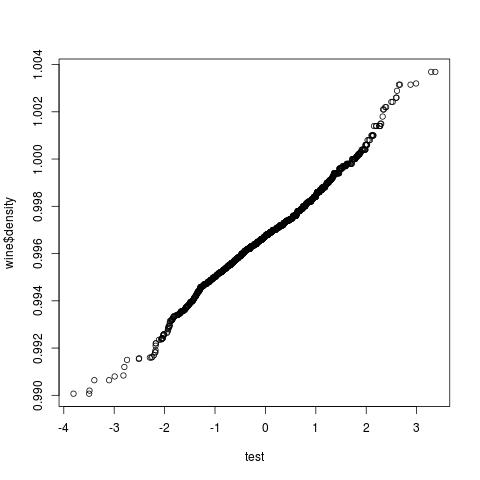
\includegraphics[width=8cm]{hw1_4c_density} \\
                However, from comparing the quantile plots with a vector of normals, it looks like possibly fixed.acidity and definitely citric.acid are not normally distributed. This means are standard error estimates will be off with a linear regression.
            \item[d)]
                Both models seem appropriate based on the usuals statistical tests. For the pH regression, we have an $R^2$ of $.2937$, with the F-test for the model and T-tests for the $\beta$s essentially yielding zero (smaller than the smallest non-zero number r can represent). Similarly, we get an $R^2$ of $.4463$ and p-values of essentially 0 for the density regression as well. However, looking at the residuals plots, it is a little less clear. 
                \\ 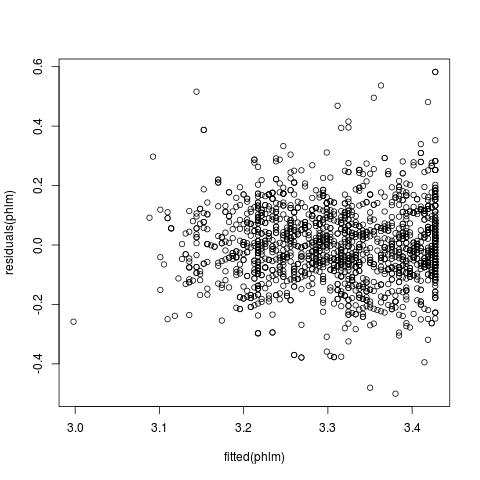
\includegraphics[width=8cm]{hw1_4d_pHresiduals} \\
                I would say the residuals for the pH model look fine, they look symmetrically distributed around 0 throughout the range of fitted values, indicating there isn't bias and that the model is alright.
                \\ 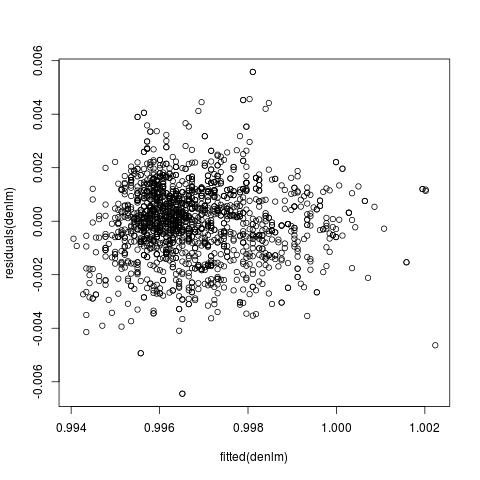
\includegraphics[width=8cm]{hw1_4d_denresiduals} \\
                However, for the density model this doesn't quite seem to be true. We seem to get a negative bias on the tails of the range of fitted values and a positive bias in the middle. This indicates that the linear model, as is, isn't appropriate.

            \item[e)]
                \\ \includegraphics[width=8cm]{hw1_4e_phfit} \\
                \\ 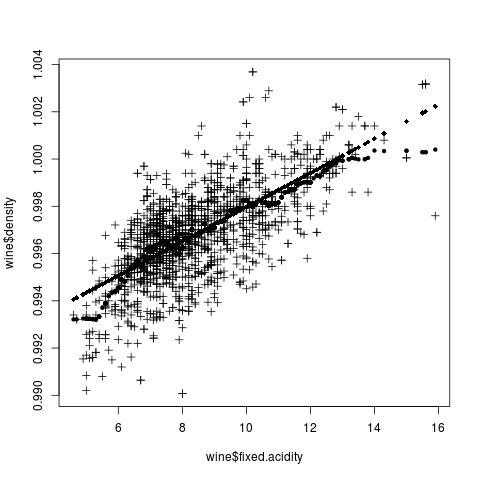
\includegraphics[width=8cm]{hw1_4e_denfit} \\
            \item[f)]
                It is clear for the pH model that the linear model (diamonds) is a better fit than the nearest neighbor model (circles), since its global  assumption of linearity appears to hold. The nearest neighbor model is essentially bouncing around the linear estimate, indicating that it merely has higher variance without capturing the underlying relationship better (it doesn't seem to have less bias). \\
 
                On the other hand, the nearest neighbor model does seem to be doing a better job on the density model. Since it is a local model that introduces less bias, it has picked up on the not quite linear (without transforming fixed.acidity anyway) relationship. The linear regression, since its global and based on a strong assumption, has introduced bias since the assumption failed.
            \item[g)]
                Considering that citric.acid is an acid, and pH is a measure for acidity, with lower values indicating higher acidity, it would stand to reason that a decrease in citric.acid would cause lower pH, as we have seen. \\
                Fixed acids seem to, in general, have much higher density than alcohol and water, which are the two main ingredients in wine. Thus, fixed acids increase the density of wine, and all else equal, one would expect higher concentrations of them would correspond to higher density.
        \end{enumerate}

\end{enumerate}

\end{document}
%%%%%%%%%%%%%%%%%%%%%%%%%%%%%%%%%%%%%%%%%%%%%%%%%%%%%%%%%%%%%%%%%%%%%%%%%%%%%%%%%%%%%%%%%%%%%%%%%%%%%%%%%%%%%%%%%%%%%%%%%%%%%%%%%%%%%

